% !TEX encoding = UTF-8 Unicode
\chapter{پژوهش‌های پیشین}\label{Chap:Chap2}

 در این فصل پژوهش‌های مرتبط  با ... 

%==================================================================
\section{مدل‌سازی انتشار رفتار}
رفتارهای اجتماعی، انتشار نُرم‌های فرهنگی و حتی اجماع بین افراد معمولا به صورت واکنش‌های دینامیکی بین مجموعه‌ای از عامل‌های به هم متصل رخ می‌دهد \cite{Vespignani2012}.  مدل‌‌سازی این دینامیک روی شبکه توجه محققان زیادی را در چند سال اخیر به خود جلب کرده است.  با توجه به ساختار شبکه و پیوستگی زمان، این مدل‌ها را می‌توان به سه دسته تقسیم کرد؛ زمان پیوسته و بدون ساختار شبکه، زمان گسسته و با ساختار شبکه، و زمان پیوسته و با ساختار شبکه.  در ادامه پژوهش‌های انجام شده در هر سه دسته آورده می‌شود.


%------------------------------------------------------------------
\subsection{زمان پیوسته و بدون ساختار شبکه}
این مدل‌ها در ابتدا برای تشخیص سرایت بیماری‌ها ارائه شده‌اند. چارچوب مدل‌های ارائه شده بر دو فرض اصلی استوار است؛ حالت
\trans{چندبخشی}{Compartmentalization}
افراد و 
\trans{ترکیب همگن}{Homogenous Mixing}   
جامعه \cite{Barabasi2015}. در مدل‌های سرایت افراد بر اساس مرحله پیشروی بیماری به حالت‌های مختلفی، مانند موارد زیر، تقسیم می‌شوند.
\begin{itemize}
	\item \trans{مستعد}{Susceptible} \lr{(S)}:
	 فرد سالمی که هنوز در معرض عامل بیماری‌زا قرار نگرفته است.
	\item  \trans{بیمار}{Infectious} \lr{(I)}: 
	فرد مبتلا به بیماری که  می‌تواند بیماری را انتقال دهد.
	\item  \trans{سالم}{Recovered} \lr{(R)}:
فردی که قبلا بیمار شده است و اکنون ناقل بیماری نیست.
\end{itemize}
ترکیب همگن افراد نیز بدین صورت است که گراف ساختار ندارد و هر فرد با احتمال یکسانی به افراد بیمار اتصال دارد. 
در واقع افراد به صورت همگن در شبکه به یکدیگر متصل هستند.
\begin{figure}
\center
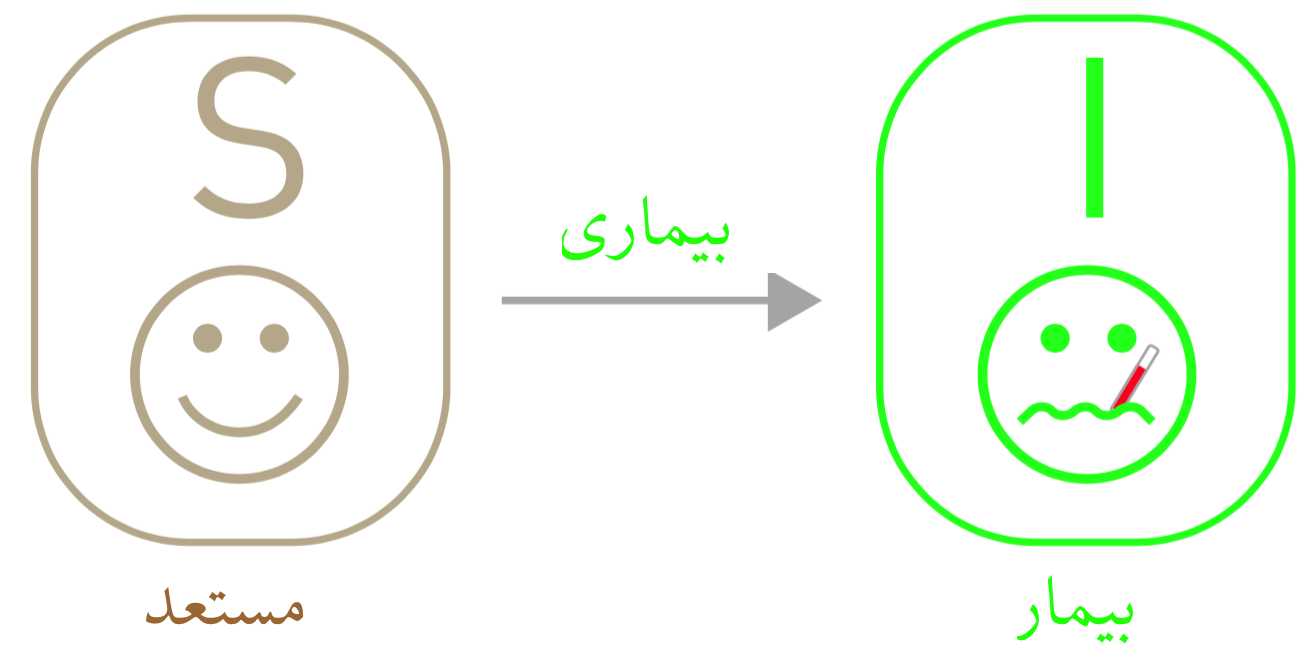
\includegraphics[width=0.3\textwidth]{images/SI_model}
\hspace{7mm}
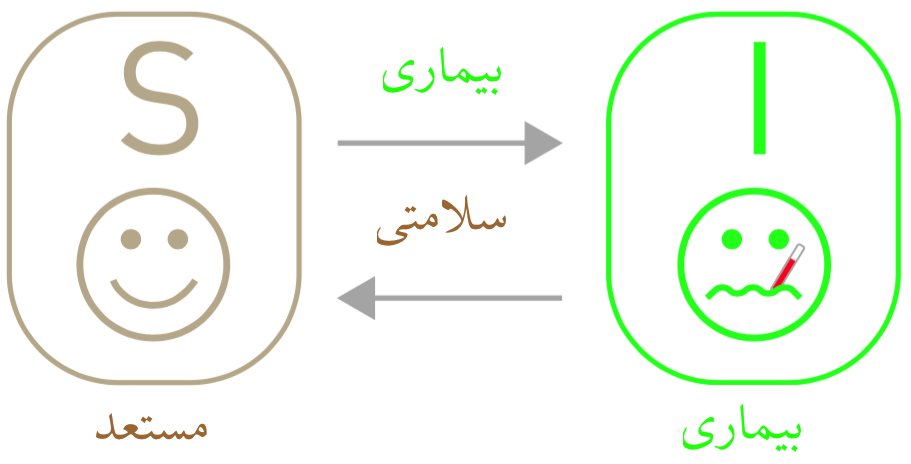
\includegraphics[width=0.3\textwidth]{images/SIS_model}\\
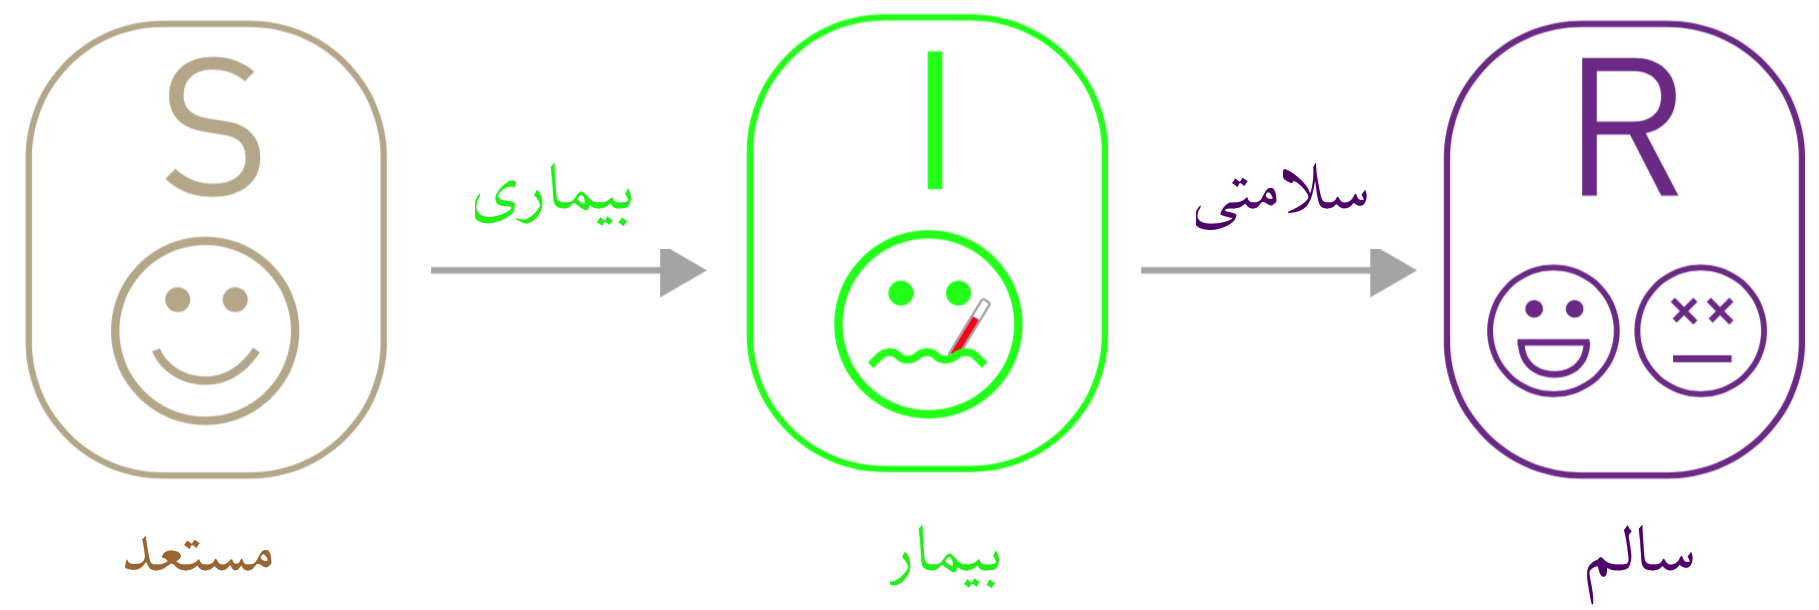
\includegraphics[width=0.5\textwidth]{images/SIR_model}
\caption{
مدل‌های سرایت \lr{SI}، \lr{SIS} و \lr{SIR} به ترتیب بالا سمت راست، بالا سمت چپ و پایین \cite{Barabasi2015}.
 }
\label{fig:epidemic-models}
\end{figure}
ساده‌ترین مدل سرایت، \lr{SI} نام دارد که...
